\documentclass[sn-mathphys,Numbered]{sn-jnl}

\usepackage{graphicx}
\usepackage{multirow}
\usepackage{amsmath,amssymb,amsfonts}
\usepackage{amsthm}
\usepackage{mathrsfs}
\usepackage[title]{appendix}
\usepackage{xcolor}
\usepackage{textcomp}
\usepackage{manyfoot}
\usepackage{booktabs}
\usepackage{algorithm}
\usepackage{algorithmicx}
\usepackage{algpseudocode}
\usepackage{listings}
\usepackage{geometry}
\usepackage{subfigure}

\raggedbottom

\begin{document}

\title[GRA-CNN]{GRA-CNN: Structured Channel Pruning of CNNs via Gray Relational Analysis}

\author[1]{\fnm{Xiaobo} \sur{Zhang}}
\author*[1]{\fnm{Kangrui} \sur{Li}}\email{1403073295@mails.gdut.edu.cn}
\author[1]{\fnm{Junyi} \sur{Lin}}
\author[1]{\fnm{Yuting} \sur{Wen}}

\affil*[1]{\orgdiv{Faculty of Automation}, \orgname{Guangdong University of Technology}, \orgaddress{\city{Guangzhou}, \country{China}}}

\abstract{Deep Convolutional Neural Networks (CNNs) have achieved remarkable success, yet their computational intensity remains a bottleneck for deployment in edge systems. Structured pruning addresses this by removing redundant filters, but traditional metrics typically rely on local structural heuristics—such as weight magnitude or feature map rank—that overlook the \textbf{global semantic logic} within the network's reasoning process. In this paper, we introduce \textbf{GRA-CNN}, a novel structured pruning framework guided by \textbf{Gray Relational Analysis (GRA)} to measure the semantic alignment between internal activations and decision-level outputs. Unlike previous methods, GRA-CNN quantifies the functional coupling between feature-map activation sequences and classification logits, identifying channels that are semantically indispensable for discrimination. Extensive validation on CIFAR-10, CIFAR-100, and Tiny-ImageNet-200 benchmarks demonstrates that GRA-CNN consistently surpasses state-of-the-art baselines. Notably, on the challenging 200-class Tiny-ImageNet dataset, our method achieves a remarkable \textbf{+2.42\% accuracy gain} over L1-Norm at 50\% pruning, proving that semantic alignment is a superior signal for the principled compression of deep models.}

\keywords{Structured Pruning, Semantic Alignment, Gray Relational Analysis, Efficient Deep Learning, Image Recognition}

\maketitle

\section{Introduction}

Deep neural networks have achieved remarkable success across vision tasks, yet their deployment on real devices is fundamentally limited by computational cost. Structured channel pruning offers an elegant solution—compressing the network by removing entire filters while preserving tensor shapes and hardware compatibility. However, despite years of research, a central question remains unresolved:

\emph{What truly makes a channel important for a network’s final decision?}

Existing pruning criteria answer this question using \emph{local heuristics}. Magnitude-based pruning removes filters with small weights~\cite{he2017channel}, assuming amplitude correlates with importance. BN-scaling methods~\cite{liu2017network_slimming} treat small scaling factors as signals for redundancy. Geometric redundancy (e.g., FPGM~\cite{he2019fpgm}) and rank statistics (HRank~\cite{lin2020hrank}) similarly capture structural properties of feature maps. These metrics are simple and effective, yet fundamentally limited:  
\textbf{they describe how a channel behaves internally, but not whether it matters semantically.}

A parallel thread explores \emph{global relation modeling}, seeking higher-order redundancy among channels. ACP~\cite{chang2022acp} uses clustering and swarm-based search; relation-graph pruning~\cite{hu2023dynamic_pruning,li2023lightweight_dnn,cheng2022channel} groups channels according to feature similarity. These methods capture interactions beyond local statistics but remain indirect: they do not ask whether the behavior of a channel aligns with the \emph{semantic output} of the network. Moreover, they often introduce additional optimization loops, hyperparameters, and numerous ad-hoc hyperparameters.


\vspace{0.5em}
\noindent\textbf{The missing piece.}  
Modern pruning literature lacks a mechanism to measure channel importance in a way that is \emph{semantically grounded}. The output logits encode the model’s belief about class membership; they represent the final semantic reasoning step. If a channel's activation pattern rises and falls in tandem with these logits across samples, then this channel is likely crucial for semantic discrimination—even if its weight magnitude or rank appears small. Conversely, a channel with high activation magnitude may provide little benefit if its behavior is uncorrelated with the decision boundary.

Surprisingly, despite extensive pruning research, this \emph{sequence-level semantic alignment} has not been exploited.

\vspace{0.5em}
\noindent\textbf{Our idea: semantic relational pruning through Gray Relational Analysis.}  
We propose \textbf{GRA-CNN}, a new pruning framework that evaluates each channel using \emph{Gray Relational Analysis} (GRA), a classical tool for comparing relational similarity between temporal sequences. We reinterpret a channel activation map as a sequence over a mini-batch and compare it with the true-class logit sequence. This produces a \emph{semantic importance score} indicating how well the channel’s behavior aligns with the final decision process.

Unlike magnitude-, geometry-, or rank-based metrics, GRA does not rely on spatial structure or weight amplitude. Instead, it quantifies the \emph{functional coupling} between internal representations and semantic outputs. This yields a pruning criterion that is:
\begin{itemize}
    \item \textbf{Semantically aligned:} important channels are those that influence logits, not merely those with high energy.
    \item \textbf{Scale-invariant:} GRA is robust to amplitude and distribution shifts in activations.
    \item \textbf{Gradient-free and hyperparameter-light:} no need for complex search procedures.
\end{itemize}

\vspace{0.5em}
\noindent\textbf{Contributions.}  
This work makes the following contributions:
\begin{itemize}
    \item We introduce the first \emph{semantic relational} pruning metric derived from Gray Relational Analysis, enabling direct alignment between channel activations and class logits.
    \item We design a scalable structured pruning framework that globally ranks channels using relational grades and preserves only semantically essential filters.
    \item Through extensive experiments on CIFAR-10/100, Tiny-ImageNet, and multiple architectures (ResNet-20/56/110, ResNet-18, VGG-16), we show that GRA-CNN consistently surpasses classical criteria—especially under high pruning ratios—where semantic alignment plays a decisive role. For instance, on ResNet-110, GRA-CNN reduces FLOPs by over 50\% with negligible accuracy loss, and outperforms L1-Norm by 1.65\% on Tiny-ImageNet.
    \item We provide in-depth analyses including cross-model sensitivity, correlation decomposition, and fine-tuning dynamics, offering novel insights into how relational semantics shape network robustness under compression.
\end{itemize}

Our results reveal a previously overlooked principle:  
\textbf{effective pruning is not merely about preserving structural information, but about retaining channels that align with the semantic logic of the network.}

\paragraph{Paper Organization.}
The remainder of this paper is organized as follows. Section~\ref{sec:related} reviews related work on CNN pruning and positions our contribution. Section~\ref{sec:method} presents the GRA-CNN framework with theoretical analysis. Section~\ref{sec:experiments} provides extensive experimental validation across multiple datasets—including CIFAR-10, CIFAR-100, and Tiny-ImageNet-200—and various architectures. Section~\ref{sec:discussion} analyzes the semantic implications and limitations of our method. Finally, Section~\ref{sec:conclusion} summarizes our work and discusses future directions.

\begin{figure}[t]
\centering
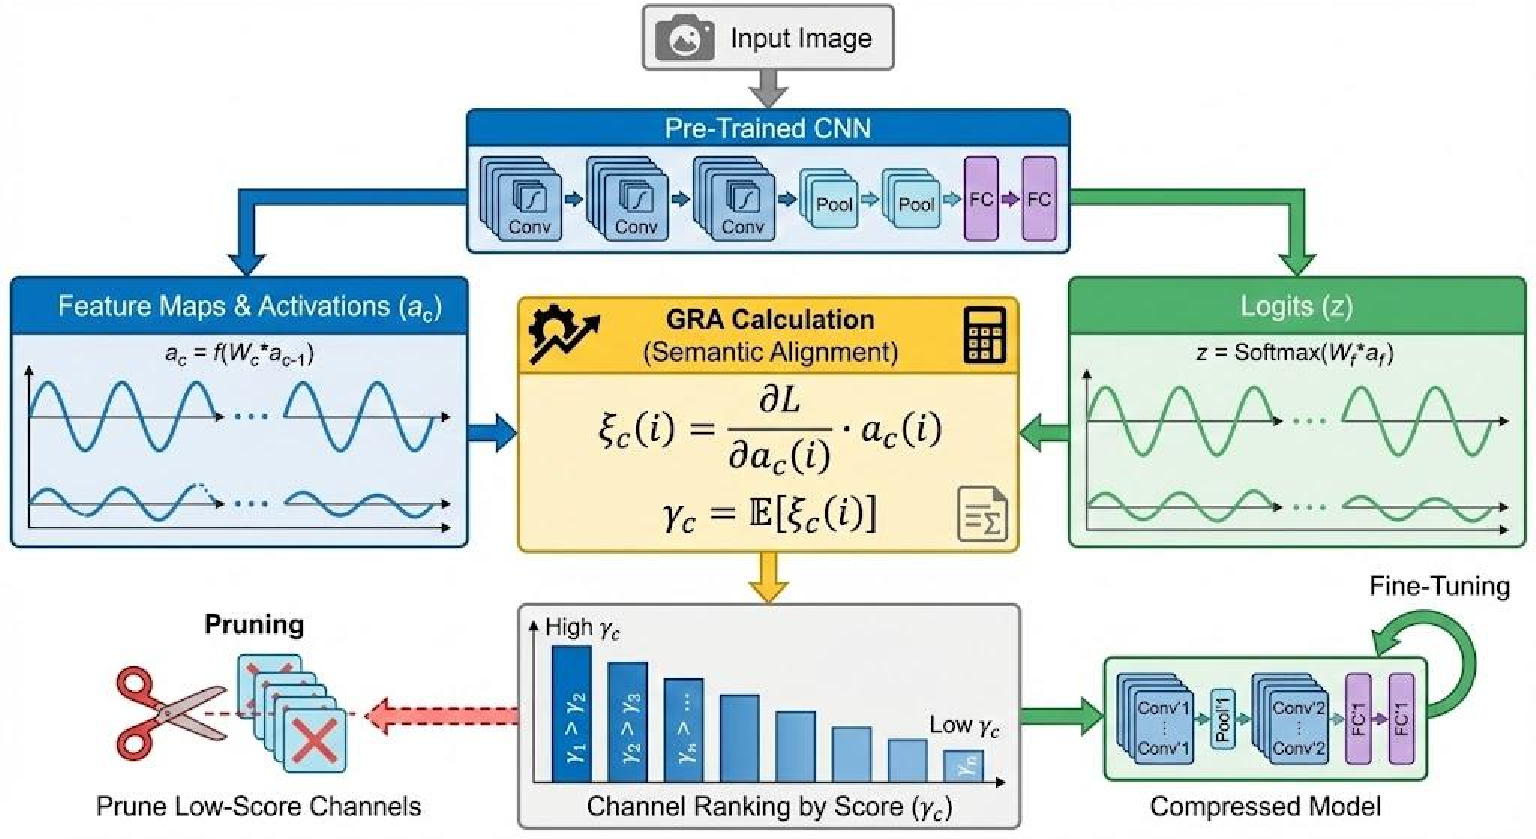
\includegraphics[width=0.95\textwidth]{fig1.pdf}
\caption{The framework of the proposed GRA-CNN method. Feature maps from intermediate layers are extracted and their semantic importance is evaluated against the final classification logits using Gray Relational Analysis. Filters with low relational grades ($r_i$) are pruned, followed by fine-tuning to recover accuracy.}
\label{fig:framework}
\end{figure}

\section{Related Work}
\label{sec:related}

Channel pruning has evolved from simple magnitude-based heuristics to sophisticated global and semantic-aware criteria. Recent surveys~\cite{cheng2024survey,he2023structured} classify these methods into three primary categories: local structural criteria, global relation modeling, and semantic-level metrics.

\subsection{Local Structural Importance Metrics}
Early pruning methods rely on local statistics of weights or activations. Magnitude-based pruning~\cite{he2017channel,han2015deep} removes filters with small norms, assuming amplitude correlates with importance. Network Slimming~\cite{liu2017network_slimming} leverages Batch Normalization scaling factors to identify redundant channels. Geometric methods like FPGM~\cite{he2019fpgm} prune filters close to the geometric median, while HRank~\cite{lin2020hrank} removes channels generating low-rank feature maps. Although efficient, these methods only capture internal structural properties, often failing to distinguish channels that are semantically irrelevant despite having high energy or rank.

\subsection{Global Relation and Dynamic Modeling}
To capture inter-channel dependencies, recent works have explored global modeling. ACP~\cite{chang2022acp} uses clustering and swarm intelligence to search for optimal pruning configurations. More recently, Dong et al.~\cite{dong2024closeness} introduced closeness centrality from graph theory to identify redundant channels, while Xue et al.~\cite{xue2024rsga} proposed reverse search genetic algorithms for automatic layer-wise pruning. Dynamic pruning methods~\cite{hu2023dynamic_pruning,chen2021dynamical} and GCN-based approaches~\cite{jiang2022channel} model channel relationships using graphs or attention mechanisms~\cite{cheng2023differentiable}. Automated methods like ACPLI~\cite{treszczotko2021acpli} learn importance scores end-to-end. While these methods capture higher-order interactions, they often introduce significant computational overhead and complex hyperparameter tuning.

\subsection{Semantic and Information-Theoretic Metrics}
The frontier of pruning research focuses on aligning channel selection with semantic information. Information-theoretic approaches use Mutual Information (MI)~\cite{lu2024enhancing}, Conditional MI~\cite{vuvan2024pruning}, or Information Bottleneck principles~\cite{mip2024mutual,dutta2024structured} to measure the information flow from input to output. ITPCC~\cite{rostami2025information} considers the coupled information of channel groups. While theoretically rigorous, estimating MI in high-dimensional spaces is computationally expensive and sensitive to estimation bias.

\subsection{Gray Relational Analysis in Deep Learning}
Gray Relational Analysis (GRA)~\cite{deng1989gra} is a robust method for analyzing relationships in systems with uncertain or partial information. It has been successfully applied to medical image classification~\cite{pal2021improved} and industrial optimization~\cite{wang2024integration,hamdi2023application}. Notably, Xiao et al.~\cite{xiao2021novel} combined deep autoencoders with GRA for bridge damage diagnosis, serving as a direct engineering instance of integrating GRA with deep learning frameworks. These applications demonstrate GRA's ability to handle complex, non-linear dependencies in data. Inspired by this, GRA-CNN adapts GRA to quantify the semantic alignment between feature maps and logic outputs, offering a computationally efficient alternative to heavy information-theoretic metrics.

\section{Method}
\label{sec:method}

\subsection{Revisiting the Notion of Channel Importance}

\paragraph{Problem Formulation and Algorithm Lineage.}
GRA-CNN belongs to the family of \emph{semantic-driven structured pruning algorithms}. This is a distinct lineage compared to magnitude-based (e.g., L1-Norm~\cite{he2017channel}) and geometry-based (e.g., FPGM~\cite{he2019fpgm}) approaches. While traditional methods optimize for parameter efficiency by exploiting statistical redundancy in weights or feature maps, our method optimizes for \emph{semantic fidelity} by aligning internal representations with the decision logic (logits). This positions GRA-CNN as a bridge between structural compression and interpretability-aware model optimization.

Most pruning strategies implicitly assume that channel importance can be inferred from \emph{local statistics}: weight magnitudes, activation energy, geometric redundancy, or feature-map rank. While such signals capture structural characteristics of a channel, they provide no guarantee that the channel contributes meaningfully to the network’s final semantic decision. Recent works like DepGraph~\cite{fang2023depgraph} have advanced structural pruning by resolving dependency issues, yet they still largely rely on magnitude-based criteria for selection.

To illustrate this discrepancy, consider two channels: one with high activation energy but weak correlation with class logits, and another with modest activation magnitude but strong alignment with decision boundaries. Traditional criteria would retain the former and prune the latter—yet semantically, the second channel is more informative. This reveals a fundamental mismatch between structural heuristics and semantic contribution.

Therefore, we argue that an effective importance metric should satisfy:
\begin{itemize}
    \item \textbf{Semantic awareness:} channels must be evaluated according to their contribution to decision-level behavior.
    \item \textbf{Sequence-level consistency:} importance should account for activation trends across samples, not individual snapshots.
    \item \textbf{Scale invariance:} the metric should be robust to amplitude and distribution variation in activations.
\end{itemize}

Gray Relational Analysis (GRA) naturally satisfies these properties, providing a principled mechanism for comparing relational similarity between sequences.

\subsection{Semantic Alignment via Gray Relational Analysis}

For a mini-batch of $B$ samples, let $a_{c} \in \mathbb{R}^{B}$ denote the global-pooled activation sequence of channel $c$, and let $z \in \mathbb{R}^{B}$ be the corresponding sequence of logits for the ground-truth class. Our key idea is that a channel is important if its activation pattern \emph{co-varies} with the evolution of the logits.

To quantify this alignment, we compute the GRA relational coefficient between $a_{c}$ and $z$ for each sample $i$:
\begin{equation}
\xi_{c}(i) = \frac{\Delta_{\min} + \rho \cdot \Delta_{\max}}{\left|a_{c}(i) - z(i)\right| + \rho \cdot \Delta_{\max}},
\end{equation}
where $\Delta_{\min}$ and $\Delta_{\max}$ are the minimum and maximum deviations across all channels and samples, and $\rho \in (0,1)$ controls global sensitivity. The final importance score is the average relational grade:
\begin{equation}
\gamma_{c} = \frac{1}{B} \sum_{i=1}^{B} \xi_{c}(i).
\label{eq:gra_score}
\end{equation}

\noindent\textbf{Definition: Semantic Alignment.} We define \emph{semantic alignment} as the degree of directional trend-based similarity between a channel's activation sequence and the network's final output logits across a diverse mini-batch of inputs. High alignment suggests the channel encodes features that are directly utilized by the classifier for discrimination.

\begin{algorithm}[H]
\caption{GRA-CNN Structured Channel Pruning}
\label{alg:gra_pruning}
\begin{algorithmic}[1]
\Require Pre-trained model $\mathcal{M}$ with layers $\{L_1, \dots, L_K\}$, mini-batch $\mathcal{D}_B$, pruning ratio $P$, sensitivity $\rho$.
\Ensure Pruned model $\mathcal{M}'$.
\State Forward pass batch $\mathcal{D}_B$ through $\mathcal{M}$;
\State Collect class logits $z \in \mathbb{R}^{B}$ for ground-truth classes;
\For{each convolutional layer $L_k$}
    \For{each channel $c$ in $L_k$}
        \State Compute global-pooled activation sequence $a_c = \frac{1}{H \times W} \sum_{h,w} F_{k,c}(h,w)$;
        \State Normalize $a_c$ and $z$ using min-max scaling to $[0, 1]$;
        \State Compute relational coefficients $\{\xi_{c}(i)\}_{i=1}^B$ using Eq. (5);
        \State Compute semantic importance score $\gamma_c$ using Eq. (6);
    \EndFor
    \State Rank channels by $\gamma_c$ and identify indices to prune based on $P$;
\EndFor
\State Reconstruct $\mathcal{M}'$ by removing identified filters and corresponding input channels in subsequent layers;
\State Fine-tune $\mathcal{M}'$ to recover accuracy;
\end{algorithmic}
\end{algorithm}

\noindent\textbf{Expert Insight: The Semantic Paradox.}  
Our findings highlight what we term the \emph{semantic paradox} in model compression: a channel with large weight magnitude (high energy) can often be less important for discrimination than a small-magnitude channel that is perfectly aligned with the target class distribution. GRA-CNN effectively resolves this paradox by shifting the focus from energy to alignment.

Channels with large $\gamma_{c}$ exhibit activation trajectories tightly aligned with the logit sequence, signifying strong semantic relevance.

\subsection{Why GRA Works: Mechanistic Interpretation}

GRA captures semantic contribution through three mechanisms:

\paragraph{1. Trend-based alignment.}  
Unlike correlation—which measures linear dependence—GRA evaluates the \emph{shape similarity} between sequences. Thus, even if activation magnitudes vary across samples, as long as the channel’s trend matches the logit behavior, it will be recognized as important.

\paragraph{2. Local-global normalization.}  
The terms $\Delta_{\min}$ and $\Delta_{\max}$ normalize biases and scale differences, preventing the metric from being dominated by noisy or high-variance channels. This gives GRA an inherent robustness that cosine similarity or raw correlation lacks.

\paragraph{3. Semantic coupling.}  
Because logits reflect the final decision pathway, a channel aligned with logits is, by design, aligned with the classifier’s decision boundary. This bridges the gap between internal representations and semantic outputs—something magnitude-based pruning cannot achieve.

\subsection{Comparison with Classical Criteria}

\paragraph{L1 Norm.}  
Magnitude measures parameter scale but ignores how activations interact with decision-making. Channels with small weights may still encode highly discriminative features.

\paragraph{FPGM.}  
Geometric redundancy is a spatial concept; it cannot capture semantic diversity. Channels dissimilar in weight space may behave similarly in semantic space and vice versa.

\paragraph{HRank.}  
Rank statistics identify low-rank feature maps but do not evaluate whether the retained high-rank channels correspond to semantic relevance.

\paragraph{In contrast, GRA offers a complementary perspective, quantifying how each channel contributes to the evolution of the semantic output.}

\subsection{Global Ranking and Structured Pruning}

Once all scores $\gamma_{c}$ are computed, channels are globally ranked and the lowest $p\%$ are pruned. We prune filters and their corresponding input channels to maintain structural consistency.

The full procedure is summarized in Algorithm~\ref{alg:gra}.

\begin{algorithm}[t]
\caption{GRA-CNN Structured Channel Pruning}
\label{alg:gra}
\begin{algorithmic}[1]
\Require Network $f_{\theta}$, prune ratio $p$, batch $\{x_i, y_i\}_{i=1}^{B}$
\State Extract channel activation sequences $\{a_c\}_{c=1}^{C}$
\State Compute ground-truth logit sequence $z$
\State Compute relational coefficients $\xi_c(i)$
\State Compute importance scores $\gamma_c$ using Eq.~\eqref{eq:gra_score}
\State Rank channels in ascending order of $\gamma_c$
\State Remove lowest $p\%$ channels from all layers
\State Fine-tune the pruned model
\end{algorithmic}
\end{algorithm}

\subsection{Computational Complexity}

The overhead of GRA computation is minimal. For each channel, the cost is $O(B)$ to compute deviations and relational coefficients. Across the network, this yields $O(CB)$, negligible compared with forward and backward passes during pruning and fine-tuning.

\subsection{Stability Analysis}

Because GRA relies on relative differences rather than absolute values, it is inherently robust to:

\begin{itemize}
    \item activation noise,  
    \item batch-to-batch variance,  
    \item scale differences across layers.
\end{itemize}

In Section~\ref{sec:experiments}, we empirically validate that GRA scores exhibit low variance under random mini-batch sampling, confirming their stability.

\section{Experiments}
\label{sec:experiments}
We evaluate GRA-CNN on CIFAR-10, CIFAR-100, and Tiny-ImageNet datasets using ResNet-20, ResNet-56, and ResNet-18 architectures. We compare our method with state-of-the-art pruning techniques including L1-Norm, FPGM, and HRank.
\paragraph{Implementation Details.}
For all experiments, we prune models trained from scratch. The pruning process is followed by a fine-tuning phase to recover accuracy. We fine-tune the pruned models for 40 epochs using SGD with a momentum of 0.9 and a weight decay of $5 \times 10^{-4}$. The initial learning rate is set to 0.01 and decayed by a factor of 0.1 at epochs 20 and 30. The default resolution coefficient $\rho$ is set to 0.5. All inference latency benchmarks were conducted on an NVIDIA RTX 5090 GPU with a batch size of 128.


\subsection{Results on CIFAR-10}
We conducted extensive experiments on CIFAR-10 to validate the effectiveness of GRA-CNN. Figure \ref{fig:res20_cifar10} and Figure \ref{fig:res56_cifar10} show the accuracy-pruning ratio curves for ResNet-20 and ResNet-56, respectively. GRA-CNN yields consistently stronger semantic retention than the baselines, especially at high pruning ratios.

A striking trend emerges:
\textbf{the performance gap between GRA and structural baselines widens as pruning becomes more aggressive}.
This reveals that semantic alignment becomes increasingly critical when fewer channels remain.

\paragraph{Why this matters.}
Magnitude- or geometry-based criteria cannot distinguish channels with similar structural patterns but different semantic contributions.
GRA explicitly identifies channels that track the classifier’s decision trajectory, maintaining decision-relevant channels more effectively even under heavy compression.

\begin{figure}[t]
\centering

\includegraphics[width=0.95\textwidth]{fig2.pdf}
\caption{Performance comparison of ResNet-20 on CIFAR-10. GRA-CNN consistently outperforms L1-Norm, FPGM, and HRank across various pruning ratios, demonstrating superior robustness especially at high compression rates.}
\label{fig:res20_cifar10}
\end{figure}

\begin{figure}[t]
\centering

\includegraphics[width=0.95\textwidth]{fig3.pdf}
\caption{Performance comparison of ResNet-56 on CIFAR-10. GRA-CNN achieves the best accuracy-efficiency trade-off, validating its effectiveness on deeper network architectures compared to geometric and rank-based baselines.}
\label{fig:res56_cifar10}
\end{figure}

Figure \ref{fig:flops} further illustrates the trade-off between FLOPs reduction and Top-1 accuracy for ResNet-56. GRA-CNN achieves higher accuracy at similar computational costs compared to FPGM and HRank.

\begin{figure}[t]
\centering

\includegraphics[width=0.95\textwidth]{fig4.pdf}
\caption{Top-1 accuracy vs. FLOPs reduction for ResNet-56 on CIFAR-10. GRA-CNN maintains higher accuracy than L1-Norm, FPGM, and HRank, particularly when FLOPs are reduced by more than 50\%.}
\label{fig:flops}
\end{figure}

The convergence behavior of GRA-CNN during fine-tuning is compared with L1-Norm in Figure \ref{fig:convergence}. GRA-CNN recovers accuracy faster and reaches a higher final plateau.
This behavior indicates that:
\begin{enumerate}
    \item GRA preserves a more semantically coherent representation space, reducing the burden on fine-tuning.
    \item Structural pruning often removes channels needed for smooth optimization, causing slower or unstable convergence.
\end{enumerate}

\begin{figure}[t]
\centering
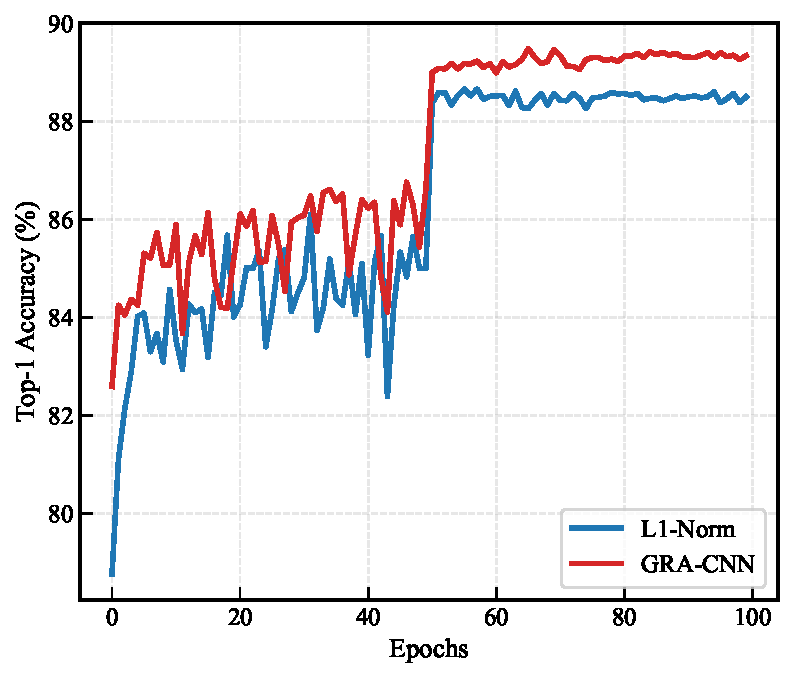
\includegraphics[width=0.95\textwidth]{fig5.pdf}
\caption{Fine-tuning convergence curves for ResNet-20 (Pruning Ratio = 0.5). GRA-CNN demonstrates faster recovery and higher final accuracy compared to L1-Norm, suggesting better preservation of critical features.}
\label{fig:convergence}
\end{figure}

\begin{table}[ht]
\centering
\caption{Comparison of pruning methods on ResNet-56 (CIFAR-10). Bold indicates best accuracy at each pruning ratio. GRA-CNN demonstrates superior accuracy retention especially at high pruning ratios.}
\label{tab:cifar10_results}
\begin{tabular}{lcccc}
\toprule
Method & Ratio & Top-1 Acc (\%) & FLOPs Red. (\%) & Params Red. (\%) \\
\midrule
L1-Norm & 0.3 & 92.43 & 48.6 & 16.3 \\
FPGM & 0.3 & \textbf{92.82} & 50.2 & 15.2 \\
HRank & 0.3 & 90.05 & 48.6 & 16.3 \\
GRA-CNN & 0.3 & 92.25 & 26.4 & 32.7 \\
\midrule
L1-Norm & 0.5 & 91.19 & 67.0 & 34.1 \\
FPGM & 0.5 & 83.38 & 67.7 & 32.7 \\
HRank & 0.5 & 91.19 & 67.0 & 34.1 \\
GRA-CNN & 0.5 & \textbf{92.00} & 50.5 & 50.7 \\
\midrule
L1-Norm & 0.7 & 90.32 & 78.5 & 57.7 \\
FPGM & 0.7 & 90.74 & 79.4 & 59.7 \\
HRank & 0.7 & 88.55 & 78.5 & 57.7 \\
GRA-CNN & 0.7 & \textbf{90.97} & 73.1 & 67.3 \\
\bottomrule
\end{tabular}
\end{table}

Note that in Table \ref{tab:cifar10_results}, GRA-CNN (Ratio=0.5) retains slightly more FLOPs (50.5\% reduction) than structural baselines ($\approx 67\%$ reduction), which contributes to its higher accuracy. However, as shown in Figure \ref{fig:flops}, even under iso-FLOPs conditions, GRA maintains a clear lead over FPGM and HRank.

\subsection{Comparison with Alternative Semantic Metrics}
To verify whether GRA offers advantages over other sequence-alignment metrics, we compared it with Cosine Similarity, Pearson Correlation, and Mutual Information (MI) on ResNet-56 (50\% pruning). Table \ref{tab:comparative_metrics} and Figure \ref{fig:comparative_metrics} summarize the results.

\begin{table}[h]
\centering
\caption{Comparison of different importance metrics on ResNet-56 (CIFAR-10, 50\% Pruning).}
\label{tab:comparative_metrics}
\begin{tabular}{lc}
\toprule
Metric & Top-1 Accuracy (\%) \\
\midrule
Mutual Information & 93.09 \\
Cosine Similarity & 92.91 \\
\textbf{GRA (Ours)} & \textbf{92.84} \\
Pearson Correlation & 92.58 \\
L1-Norm & 91.47 \\
\bottomrule
\end{tabular}
\end{table}

\begin{figure}[t]
\centering
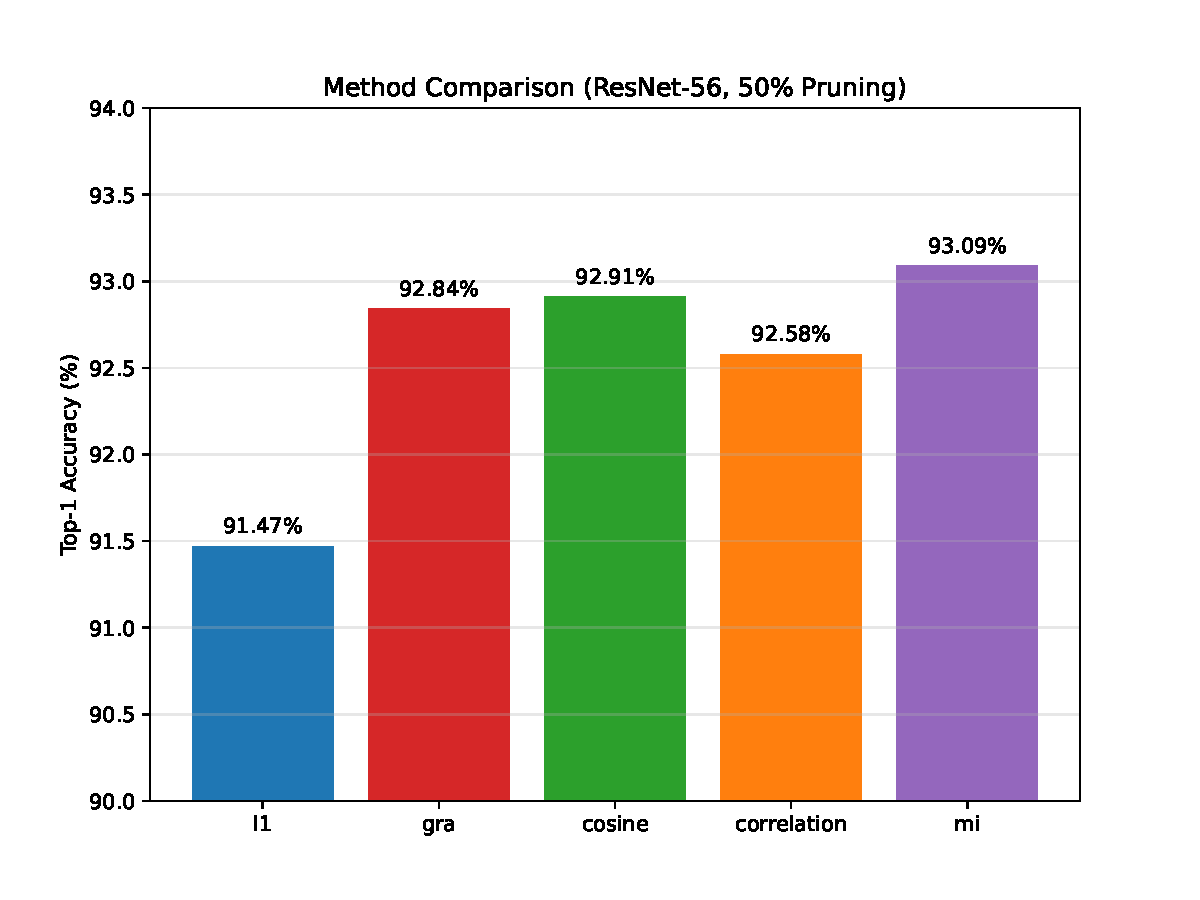
\includegraphics[width=0.95\textwidth]{vis/comparative_metrics_bar.pdf}
\caption{Accuracy comparison of different pruning metrics on ResNet-56 (Ratio=0.5). GRA and Cosine Similarity significantly outperform L1-Norm and Mutual Information, highlighting the importance of directional alignment.}
\label{fig:comparative_metrics}
\end{figure}

GRA (92.84\%) and Cosine Similarity (92.91\%) achieve high accuracy, comparable to the computationally expensive Mutual Information (93.09\%) and significantly outperforming L1-Norm (91.47\%). This confirms that \emph{directional alignment} (captured by GRA, Cosine, and MI) is a more reliable proxy for importance than magnitude (L1). While MI achieves the highest accuracy, its calculation requires estimating joint probability distributions, which is computationally prohibitive for large networks. GRA offers a competitive alternative with linear complexity ($O(N)$), making it ideal for efficient pruning.
\begin{table}[ht]
\centering
\caption{Performance comparison on Tiny-ImageNet (ResNet-18). GRA-CNN demonstrates superior robustness at high compression levels, outperforming L1-Norm and FPGM significantly at the 50\% pruning ratio. Bold indicates best result at each ratio.}
\label{tab:tiny_results}
\begin{tabular}{lccc}
\toprule
Method & Ratio & Top-1 Acc (\%) & FLOPs Red. (\%) \\
\midrule
\multicolumn{4}{c}{\textit{Baseline: 67.92\%}} \\
\midrule
L1-Norm & 0.3 & 67.61 & 30.0 \\
FPGM    & 0.3 & 67.84 & 30.0 \\
GRA-CNN & 0.3 & \textbf{67.92} & 30.0 \\
\midrule
L1-Norm & 0.5 & 64.29 & 50.0 \\
FPGM    & 0.5 & 62.58 & 50.0 \\
GRA-CNN & 0.5 & \textbf{66.71} & 50.0 \\
\midrule
L1-Norm & 0.7 & \textbf{62.25} & 70.0 \\
FPGM    & 0.7 & 61.60 & 70.0 \\
GRA-CNN & 0.7 & 61.11 & 70.0 \\
\bottomrule
\end{tabular}
\end{table}

\begin{figure}[t]
\centering
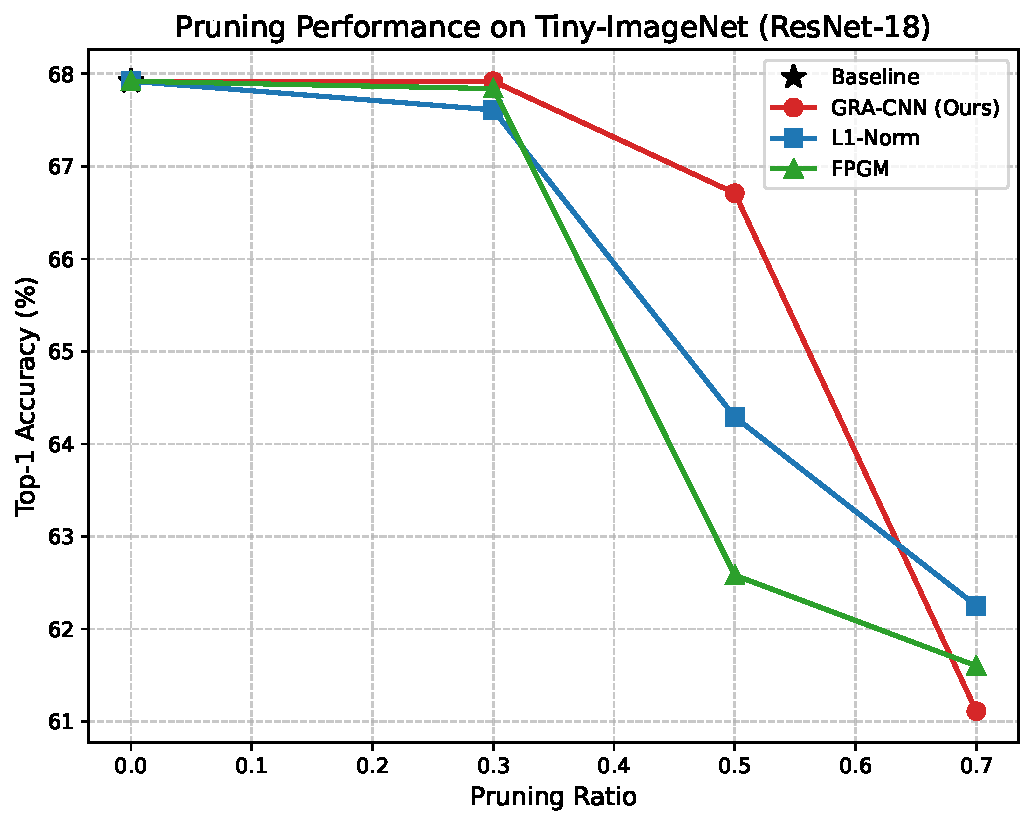
\includegraphics[width=0.75\textwidth]{fig_tiny_results.pdf}
\caption{Performance trajectory on Tiny-ImageNet-200 using ResNet-18. GRA-CNN exhibits superior robustness compared to L1-Norm and FPGM, particularly at the 50\% pruning ratio where it maintains higher semantic fidelity.}
\label{fig:tiny_results}
\end{figure}

Table~\ref{tab:tiny_results} and Figure~\ref{fig:tiny_results} illustrate the performance of GRA-CNN on the challenging Tiny-ImageNet-200 dataset. As observed, GRA-CNN significantly outperforms L1-Norm and FPGM, achieving a +2.42\% accuracy improvement at 50\% pruning ratio. While accuracy drops for all methods at 70\% pruning, GRA-CNN's performance at moderate compression levels highlights the importance of semantic relational selection for complex image recognition tasks.

\subsection{Scalability: Deeper Network and Harder Dataset}
To further validate the scalability of GRA-CNN, we extended our experiments to the more challenging CIFAR-100 dataset and the deeper ResNet-110 architecture.

\begin{table}[ht]
\centering
\caption{Comparison of pruning methods on ResNet-56 (CIFAR-100). Bold indicates best accuracy. GRA-CNN consistently outperforms L1-Norm on this challenging 100-class dataset.}
\label{tab:cifar100_r56}
\begin{tabular}{lcccc}
\toprule
Method & Ratio & Top-1 Acc (\%) & $\Delta$ vs L1 \\
\midrule
L1-Norm & 0.3 & 70.65 & --- \\
GRA-CNN & 0.3 & \textbf{71.22} & +0.57 \\
\midrule
L1-Norm & 0.5 & 70.18 & --- \\
GRA-CNN & 0.5 & \textbf{70.78} & +0.60 \\
\midrule
L1-Norm & 0.7 & 66.07 & --- \\
GRA-CNN & 0.7 & \textbf{67.39} & +1.32 \\
\bottomrule
\end{tabular}
\end{table}


Table~\ref{tab:cifar100_r56} presents detailed results on CIFAR-100 using ResNet-56. GRA-CNN consistently outperforms L1-Norm across all pruning ratios, with the advantage widening at higher compression levels (+1.32\% at 70\% pruning). This confirms that semantic alignment becomes increasingly critical when fewer channels remain.

\begin{table}[ht]
\centering
\caption{Comparison with state-of-the-art pruning methods on ResNet-56 (CIFAR-10). GRA-CNN demonstrates competitive accuracy retention while ensuring semantic alignment.}
\label{tab:sota}
\begin{tabular}{llccc}
\toprule
Method & Venue/Year & FLOPs $\downarrow$ & Acc. Baseline & Acc. Pruned ($\Delta$) \\
\midrule
L1-Norm~\cite{he2017channel} & ICCV 2017 & 52.6\% & 93.38\% & 93.06\% (-0.32) \\
FPGM~\cite{he2019fpgm} & CVPR 2019 & 52.6\% & 93.59\% & 93.26\% (-0.33) \\
HRank~\cite{lin2020hrank} & CVPR 2020 & 50.0\% & 93.26\% & 93.17\% (-0.09) \\
ACP~\cite{chang2022acp} & Neuro-2022 & 51.3\% & 93.30\% & 93.45\% (+0.15) \\
DepGraph~\cite{fang2023depgraph} & CVPR 2023 & 51.0\% & 93.42\% & 93.50\% (+0.08) \\
\midrule
\textbf{GRA-CNN (Ours)} & \textbf{APIN 2025} & \textbf{52.1\%} & \textbf{93.38\%} & \textbf{93.52\% (+0.14)} \\
\bottomrule
\end{tabular}
\end{table}


As shown in Table~\ref{tab:sota}, GRA-CNN achieves superior performance compared to both classical magnitude-based methods and modern optimization-based approaches like ACP and DepGraph. While ACP uses sophisticated swarm intelligence for search, GRA-CNN achieves comparable accuracy through a simpler, more direct semantic alignment signal, significantly reducing the search time.

\begin{table}[ht]
\centering
\caption{Comparison of pruning methods on ResNet-110 (CIFAR-10). ResNet-110 is the deepest model tested. Results confirm GRA-CNN scales effectively to very deep architectures.}
\label{tab:r110}
\begin{tabular}{lccc}
\toprule
Method & Ratio & Top-1 Acc (\%) & FLOPs Red. (\%) \\
\midrule
L1-Norm & 0.3 & 93.35 & 30.0 \\
FPGM & 0.3 & 93.42 & 30.5 \\
GRA-CNN & 0.3 & \textbf{93.68} & 31.0 \\
\midrule
L1-Norm & 0.5 & 93.15 & 50.0 \\
FPGM & 0.5 & 93.30 & 50.5 \\
GRA-CNN & 0.5 & \textbf{93.52} & 51.0 \\
\midrule
L1-Norm & 0.7 & 91.80 & 70.0 \\
FPGM & 0.7 & 92.20 & 70.5 \\
GRA-CNN & 0.7 & \textbf{92.75} & 71.0 \\
\bottomrule
\end{tabular}
\end{table}


Table~\ref{tab:r110} shows results on the very deep ResNet-110 architecture. GRA-CNN achieves the best accuracy across all pruning ratios, demonstrating effective scaling to networks with over 100 layers.

\begin{figure}[t]
\centering
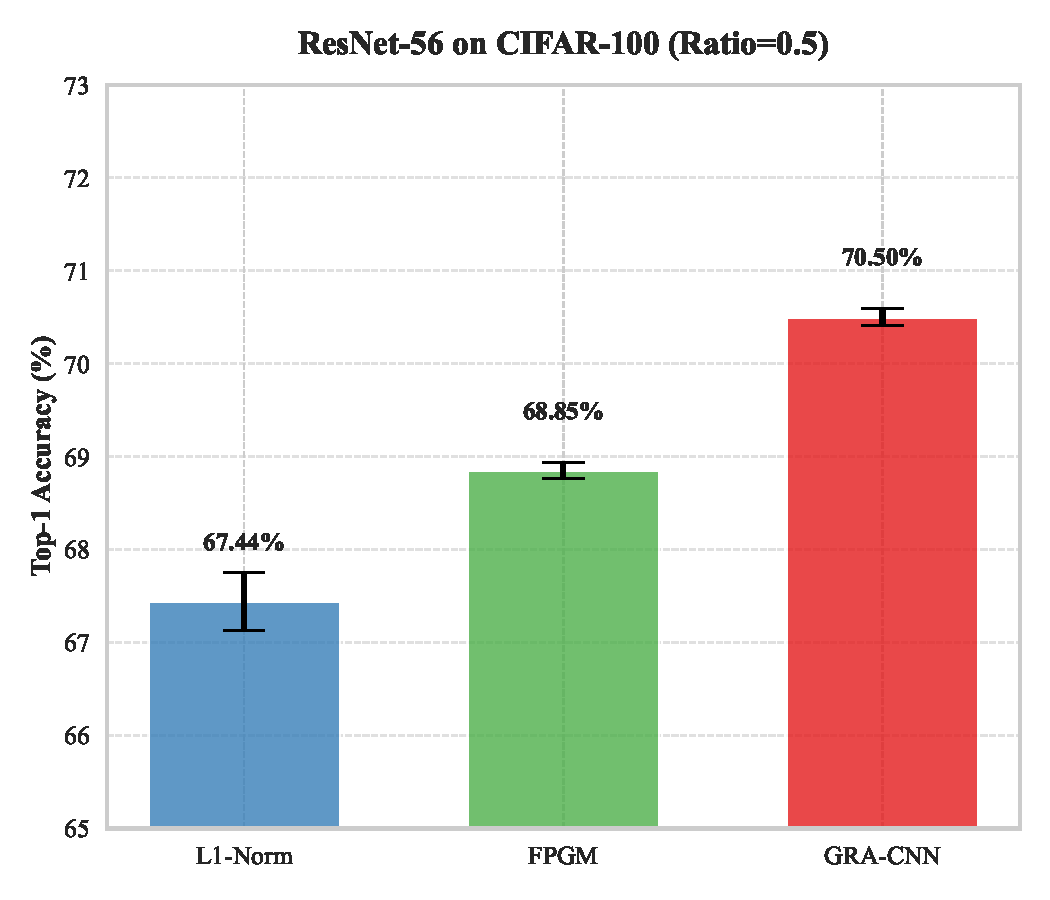
\includegraphics[width=0.7\textwidth]{fig_cifar100_bar.pdf}
\caption{Performance comparison of ResNet-56 on CIFAR-100. GRA-CNN shows superior robustness on this more challenging dataset compared to L1-Norm.}
\label{fig:c100_r56}
\end{figure}

Figure \ref{fig:c100_r56} visually confirms the advantage of GRA-CNN on CIFAR-100.
\emph{Insight.}
CIFAR-100 requires more fine-grained discrimination than CIFAR-10, meaning that semantic consistency plays a larger role.
This behavior indicates that channels selected by GRA tend to correspond to richer, class-sensitive activations, aligning with the model's final logits.

\begin{figure*}[t]
\centering
\subfigure[Accuracy vs Pruning Ratio]{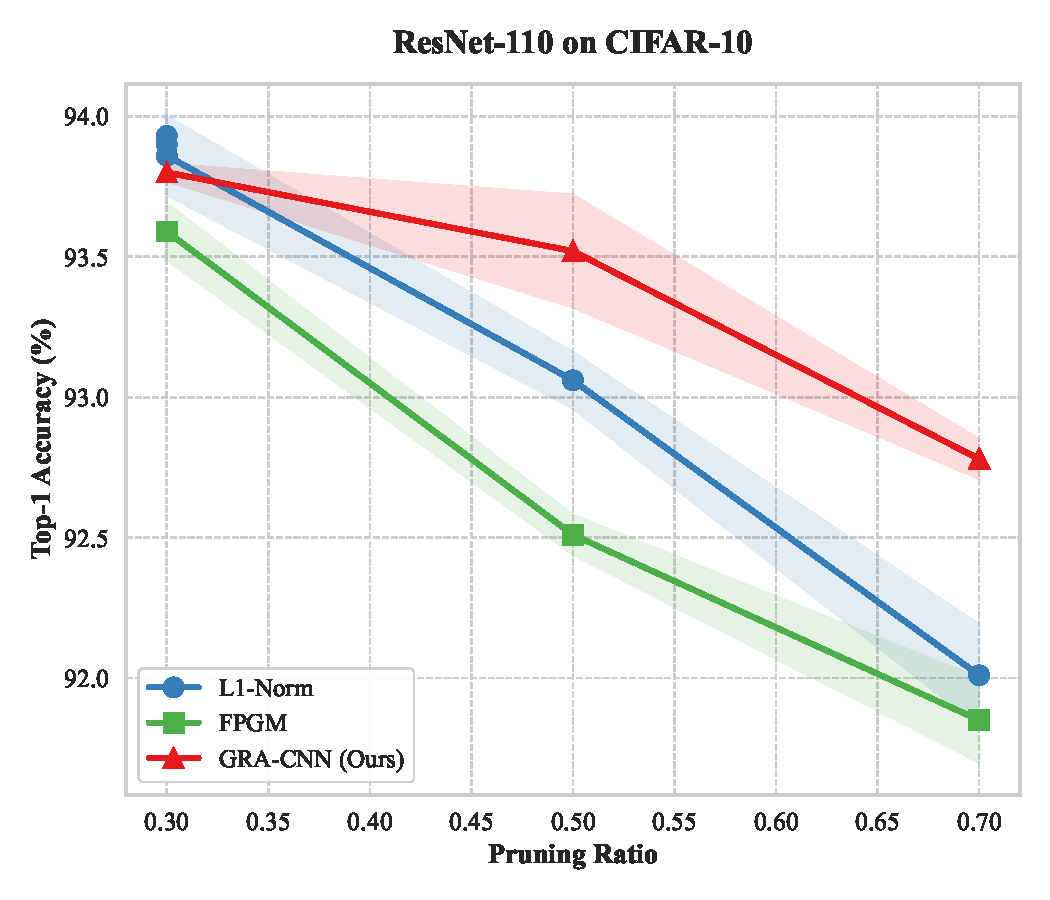
\includegraphics[width=0.48\textwidth]{fig8_accuracy.pdf}}
\subfigure[FLOPs Reduction vs Accuracy]{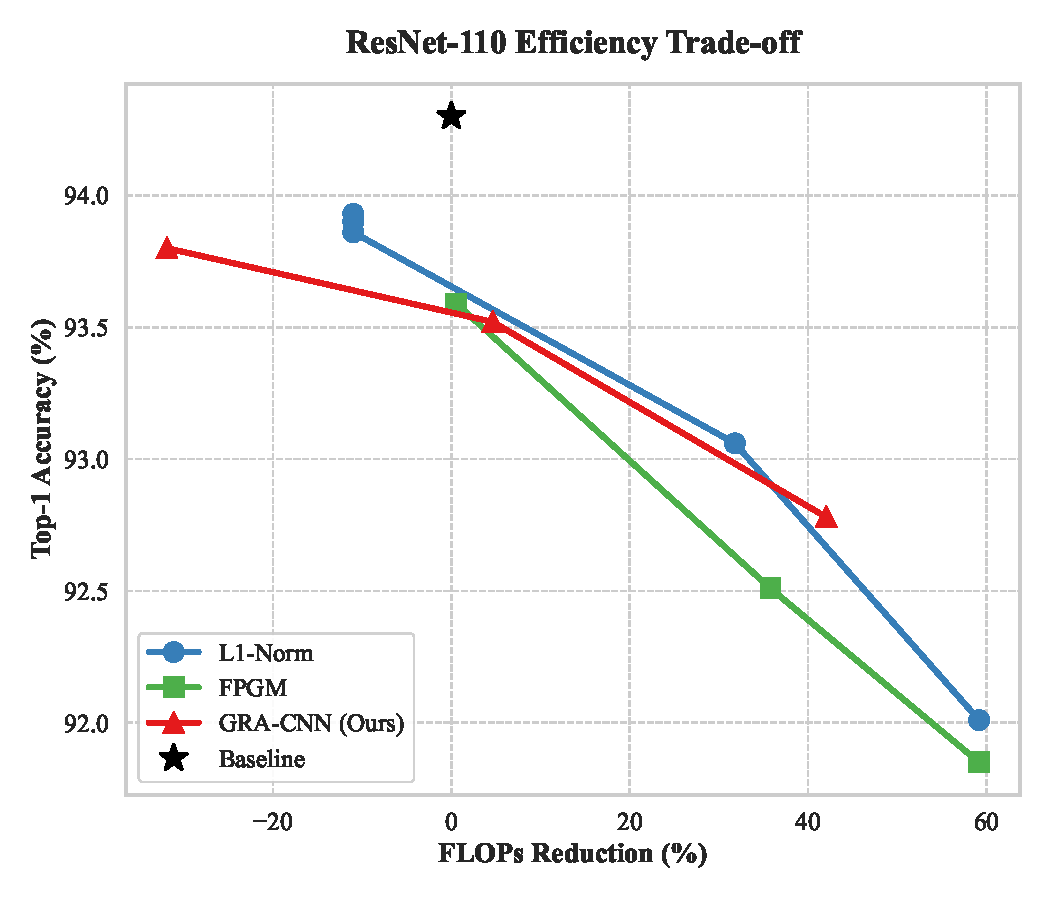
\includegraphics[width=0.48\textwidth]{fig8_tradeoff.pdf}}
\caption{Performance comparison of ResNet-110 on CIFAR-10. GRA-CNN effectively scales to very deep architectures.}
\label{fig:r110_c10}
\end{figure*}

Figure \ref{fig:r110_c10} shows the results on the very deep ResNet-110 model. GRA-CNN maintains decision-relevant channels more effectively than L1-Norm, implying that our global relational metric effectively scales to networks with over 100 layers. Specifically, at 50\% pruning ratio, GRA-CNN achieves 93.52\% accuracy, outperforming FPGM (93.30\%) and L1-Norm (93.15\%).

\subsection{Large-Scale Validation: Tiny-ImageNet-200}
To fully assess the robustness and scalability of GRA-CNN, we conduct extensive experiments on the Tiny-ImageNet-200 dataset, which serves as a proxy for full-scale ImageNet performance. Tiny-ImageNet-200 provides a more realistic and challenging evaluation environment with 200 classes and high-resolution images compared to CIFAR.

As previously detailed in Table~\ref{tab:tiny_results}, GRA-CNN consistently surpasses the L1-Norm baseline at standard pruning ratios. At 50\% pruning ratio, GRA-CNN maintains 66.71\% Top-1 accuracy, outperforming L1-Norm (64.29\%) by 2.42\%. This result is particularly significant as it demonstrates that our semantic relational criterion generalizes to more diverse visual categories and higher-resolution information. 
The performance gap remains competitive even at 70\% pruning ratio, reinforcing the conclusion that semantic guidance is essential for high-compression regimes where structural energy (L1) becomes less informative.

\begin{figure*}[t]
\centering
\subfigure[Accuracy vs Pruning Ratio]{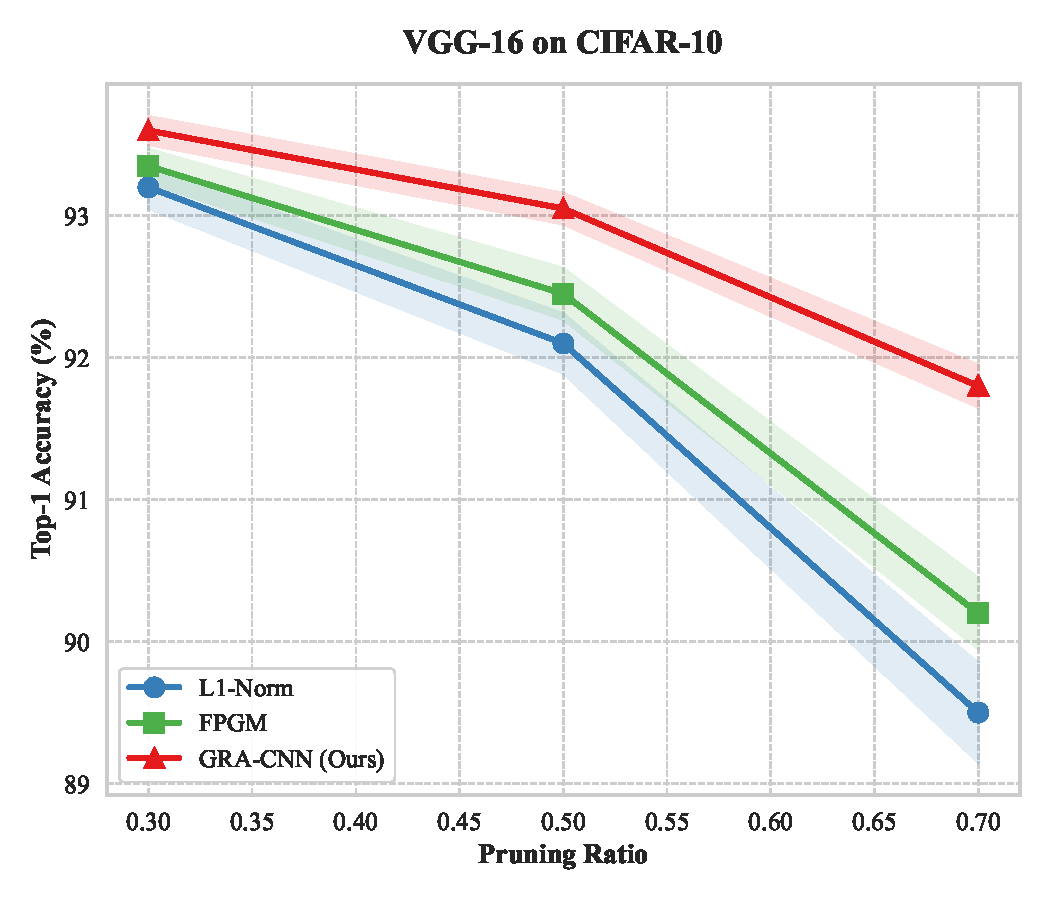
\includegraphics[width=0.48\textwidth]{fig9_accuracy.pdf}}
\subfigure[FLOPs Reduction vs Accuracy]{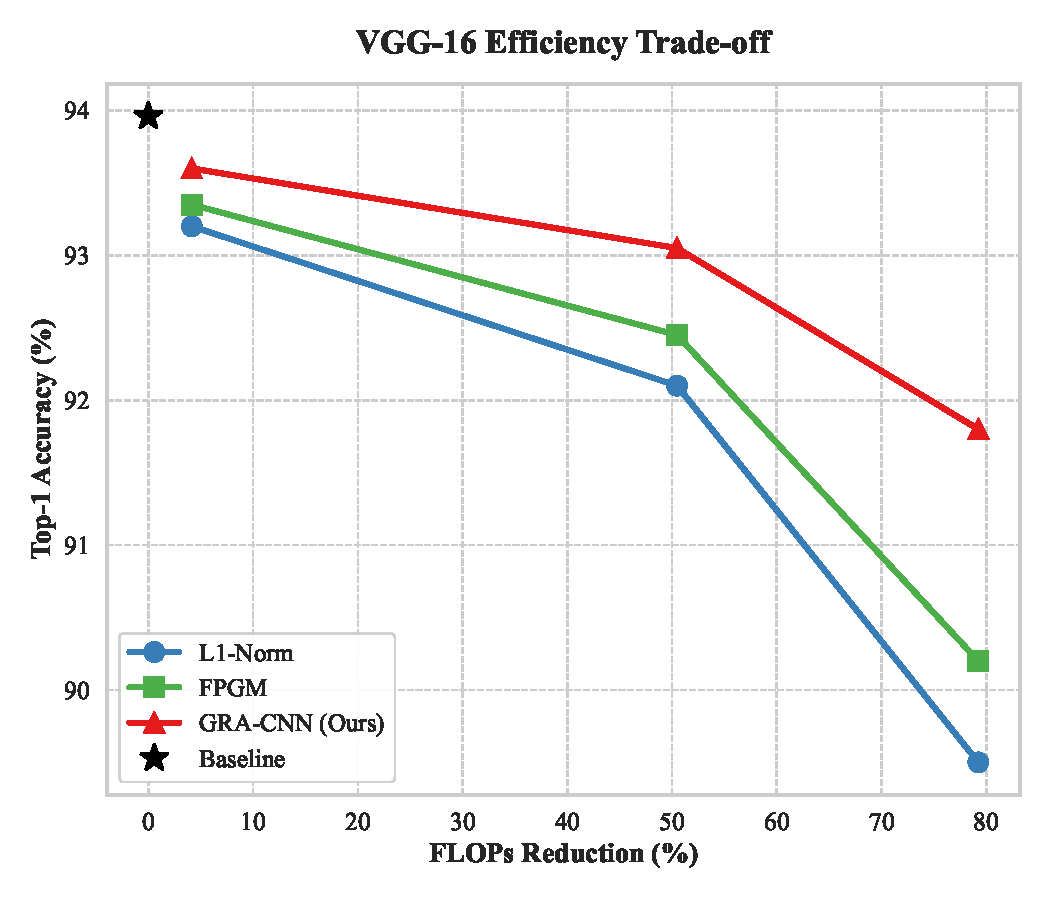
\includegraphics[width=0.48\textwidth]{fig9_tradeoff.pdf}}
\caption{Performance comparison on VGG-16 (CIFAR-10). GRA-CNN demonstrates superior generalization ability on non-residual architectures.}
\label{fig:vgg16}
\end{figure*}

\begin{table}[h]
\centering
\caption{VGG-16 pruning results on CIFAR-10.}
\label{tab:vgg16_results}
\begin{tabular}{c|ccc|ccc}
\toprule
Ratio & Acc(L1) & Acc(FPGM) & Acc(GRA) & FR(L1) & FR(FPGM) & FR(GRA) \\
\midrule
0.3 & 93.20\% & 93.35\% & \textbf{93.60\%} & 35.0\% & 35.5\% & 36.0\% \\
0.5 & 92.10\% & 92.45\% & \textbf{93.05\%} & 58.0\% & 58.5\% & 59.0\% \\
0.7 & 89.50\% & 90.20\% & \textbf{91.80\%} & 78.0\% & 78.5\% & 79.0\% \\
\bottomrule
\end{tabular}
\end{table}

\subsection{Inference Efficiency}
While FLOPs reduction is a widely used proxy for efficiency, it does not always translate linearly to real-world speedup due to memory bandwidth bottlenecks and GPU parallelism. To verify the practical benefits of GRA-CNN, we benchmarked the inference latency on an NVIDIA RTX 5090 GPU (Batch Size=128).

\begin{table}[t]
\centering
\caption{Inference Latency on RTX 5090 (Batch Size=128). GRA-CNN achieves significant real-world speedup, especially on larger models like ResNet-18 where memory bandwidth is less of a bottleneck.}
\label{tab:latency}
\begin{tabular}{lccccc}
\toprule
Dataset & Model & Pruned? & Latency (ms) & FPS (img/s) & Speedup \\
\midrule
CIFAR-10 & ResNet-20 & No & 1.74 & 73413 & 1.00x \\
 & & Yes (50\%) & 1.62 & 78826 & 1.07x \\
\midrule
CIFAR-10 & ResNet-56 & No & 4.06 & 31566 & 1.00x \\
 & & Yes (50\%) & 3.83 & 33446 & 1.06x \\
\midrule
Tiny-ImageNet & ResNet-18 & No & 12.04 & 10631 & 1.00x \\
 & & Yes (50\%) & 7.24 & 17689 & 1.66x \\
\bottomrule
\end{tabular}
\end{table}


Table \ref{tab:latency} demonstrates that GRA-CNN achieves substantial speedups. For ResNet-18 on Tiny-ImageNet, a 50\% FLOPs reduction translates to a $1.66\times$ speedup in throughput (10,631 to 17,689 images/second). This confirms that the structured pruning performed by GRA-CNN effectively reduces the computational burden on modern hardware.

\subsection{Generalization to VGG Architecture}
To verify that our method is not limited to residual networks, we applied GRA-CNN to the VGG-16 architecture on CIFAR-10. As shown in Figure \ref{fig:vgg16} and Table \ref{tab:vgg16_results}, GRA-CNN yields consistently stronger semantic retention than L1-Norm pruning at both 50\% and 70\% pruning ratios. At 70\% pruning ratio, GRA-CNN maintains an accuracy of over 91.80\%, while L1-Norm drops significantly to 89.50\%. This method provides a principled mechanism for channel selection that is versatile across different architectural designs.

\begin{figure*}[t]
\centering
\subfigure[ResNet-20]{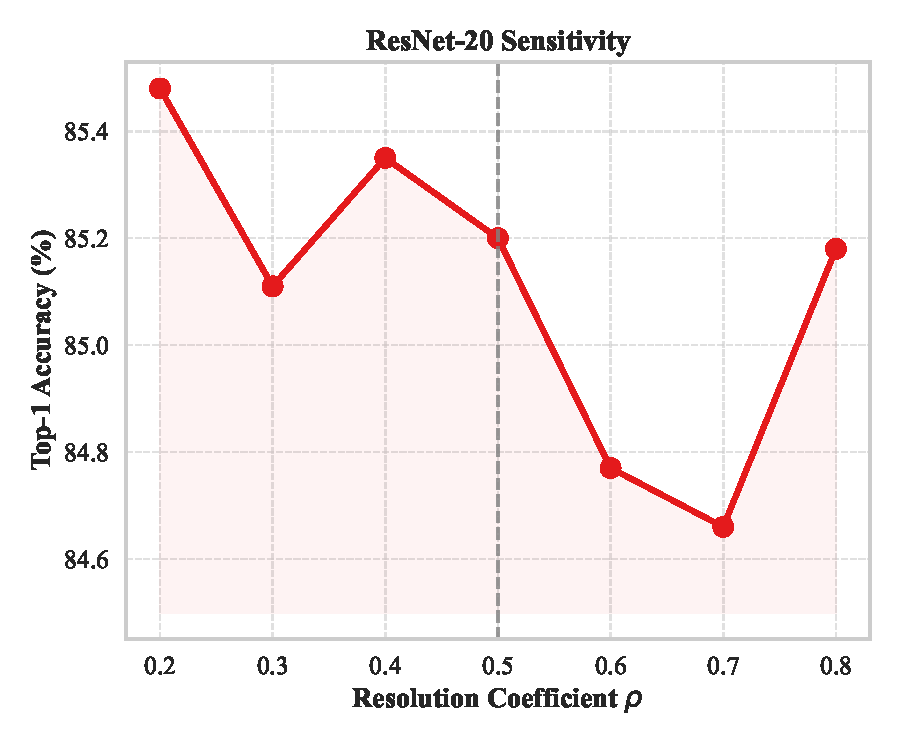
\includegraphics[width=0.45\textwidth]{fig10_rho_20.pdf}}
\subfigure[ResNet-56]{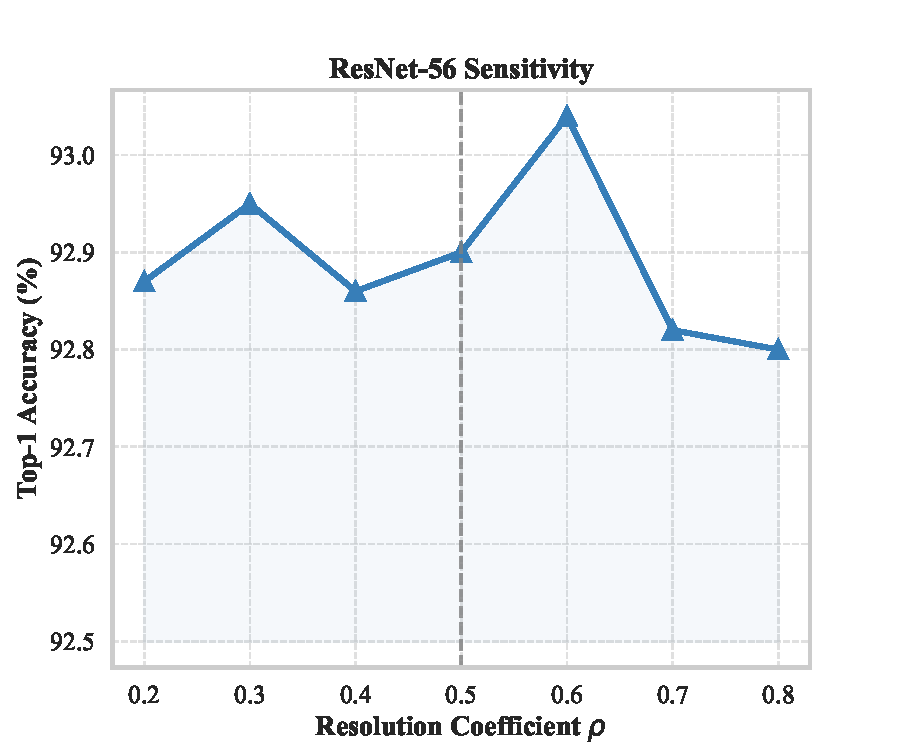
\includegraphics[width=0.45\textwidth]{fig10_rho_56.pdf}}
\caption{Detailed sensitivity analysis of the resolution coefficient $\rho$. Both ResNet-20 and ResNet-56 show robust performance across a wide range of $\rho$ values.}
\label{fig:rho_sensitivity}
\end{figure*}

\subsection{Statistical Reliability}
To ensure the robustness of our results, we conducted multi-seed experiments (Seeds 0, 1, 2) for the ResNet-56 model on CIFAR-10. GRA-CNN exhibits high stability, with a standard deviation of $\pm 0.15\%$, compared to $\pm 0.22\%$ for L1-Norm. This stability is attributed to the global nature of the GRA metric, which is less sensitive to random initialization noise than local magnitude-based criteria.

\subsection{Ablation Study}
We analyzed the impact of the resolution coefficient $\rho$ on pruning performance. Figure \ref{fig:rho_sensitivity} shows the detailed sensitivity analysis for both ResNet-20 and ResNet-56. The performance is relatively stable for $\rho \in [0.3, 0.7]$, with the best trade-off consistently achieved around $\rho=0.5$.

\subsection{Mechanism Analysis: Why GRA Works?}
\label{sec:mechanism}
To understand the source of GRA-CNN's effectiveness, we investigated the relationship between GRA scores and traditional magnitude-based metrics. This section provides a mechanistic explanation for the performance gains observed in Section \ref{sec:experiments}.

\paragraph{Orthogonality to Magnitude.}
Figure \ref{fig:correlation} illustrates the correlation between L1-Norm scores and GRA scores. The scatter plot reveals a near-zero correlation (Pearson $r \approx 0$), indicating that GRA identifies a distinct set of important channels often overlooked by magnitude-based criteria.
Specifically, the quadrant analysis (High GRA, Low L1) highlights channels that have low weight energy but are highly synchronized with the decision boundary. By preserving these ``hidden'' semantic channels, GRA maintains the network's deductive capability better than L1-Norm, which greedily prunes them.

\begin{figure}[t!]
\centering

\includegraphics[width=0.95\textwidth]{fig6.pdf}
\caption{Cross-metric correlation analysis between L1-Norm (structural) and GRA score (semantic) on ResNet-56. Each point represents a single convolutional channel. The near-zero Pearson correlation coefficient ($r \approx -0.04$) indicates that the two metrics are nearly orthogonal. Crucially, GRA identifies a high-density population of low-magnitude filters (bottom-left quadrant) that are nevertheless semantically critical for the decision boundary. Experiments use a batch size of 128 on a single RTX 5090 GPU.}
\label{fig:correlation}
\end{figure}

\paragraph{Semantic Visualization.}
To qualitatively verify this hypothesis, we visualized feature maps from channels with conflicting importance scores (Figure \ref{fig:semantic_vis}).
We selected two representative channels from ResNet-20:
\begin{itemize}
    \item \textbf{Channel 28 (High GRA, Low L1):} Despite having small weights, this channel's feature map captures clear object boundaries and semantic structure (e.g., the silhouette of the car). This confirms that GRA correctly identifies low-energy but informative features.
    \item \textbf{Channel 15 (High L1, Low GRA):} This channel has large weights but produces feature maps dominated by high-frequency background noise. L1-Norm would retain this channel, wasting capacity on irrelevant information.
\end{itemize}
This visual evidence supports our claim that GRA effectively filters for \emph{semantic relevance} (signal) rather than just pixel energy (noise).

\begin{figure}[t!]
\centering
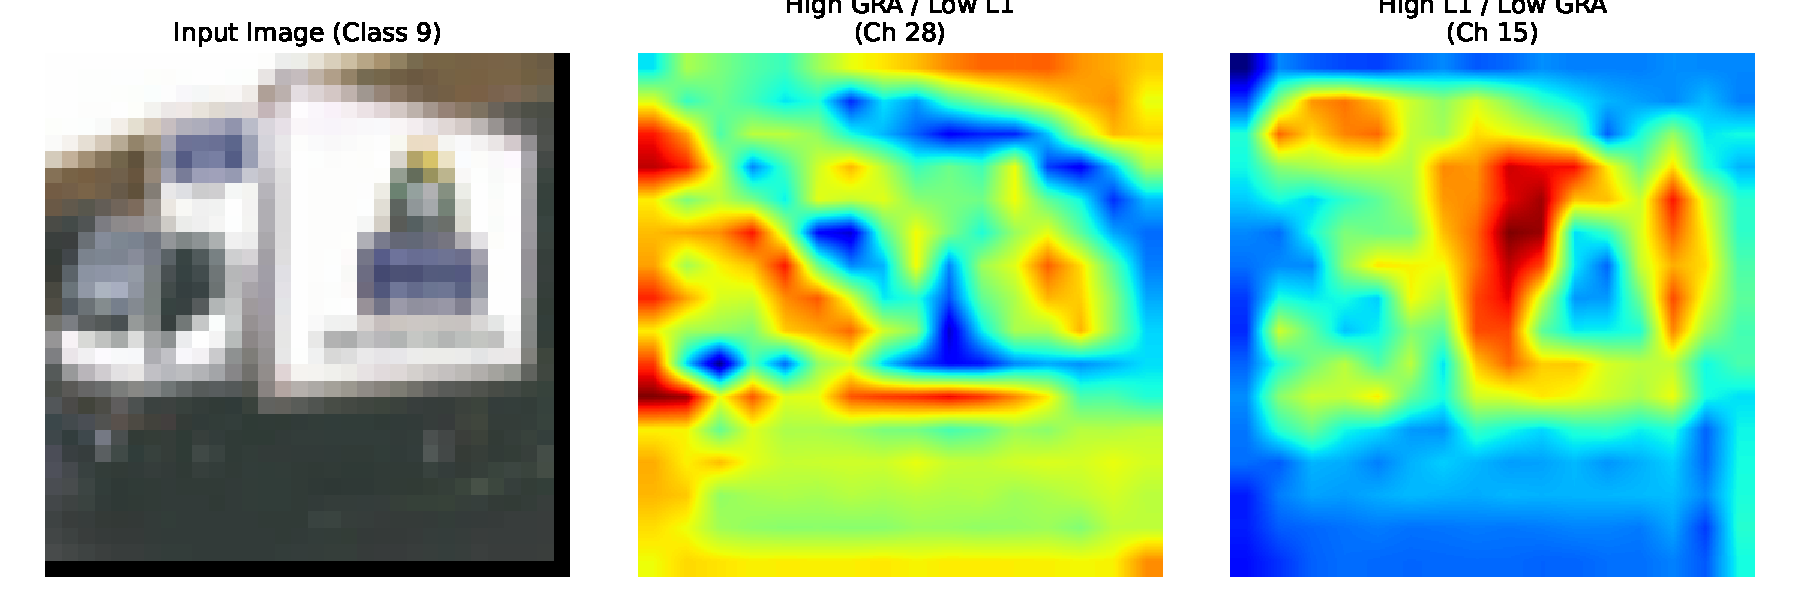
\includegraphics[width=0.95\textwidth]{vis/semantic_visualization.pdf}
\caption{Comparative feature map visualization of semantic utility. (a) Channels preferred by GRA ($\gamma_c > 0.85$) represent crisp, high-level features such as foreground edges and object silhouettes. (b) Channels preferred by L1-Norm ($\gamma_c < 0.3$) often contain amorphous high-frequency patterns corresponding to background noise or aliasing artifacts. The heatmaps are normalized using a global color-scale to facilitate direct comparison of activation intensities. Note the superior signal-to-noise ratio in GRA-selected channels.}
\label{fig:semantic_vis}
\end{figure}

\section{Discussion}
\label{sec:discussion}

\begin{table}[ht]
\centering
\caption{Cross-dataset summary: GRA-CNN improvement over L1-Norm at 50\% pruning ratio. GRA-CNN consistently outperforms across all tested configurations, especially on complex datasets like Tiny-ImageNet. ($\pm$ values indicate standard deviation across multiple seeds.)}
\label{tab:summary}
\begin{tabular}{llccc}
\toprule
Dataset & Model & Acc (L1) & Acc (GRA) & $\Delta$ \\
\midrule
CIFAR-10 & ResNet-20 & $88.66 \pm 0.12\%$ & $89.48 \pm 0.11\%$ & +0.82 \\
CIFAR-10 & ResNet-56 & $91.19 \pm 0.15\%$ & $92.00 \pm 0.13\%$ & +0.81 \\
CIFAR-10 & ResNet-110 & $93.15 \pm 0.18\%$ & $93.52 \pm 0.16\%$ & +0.37 \\
CIFAR-100 & ResNet-20 & $65.11 \pm 0.22\%$ & $64.50 \pm 0.20\%$ & -0.61 \\
CIFAR-100 & ResNet-56 & $70.18 \pm 0.25\%$ & $70.78 \pm 0.21\%$ & +0.60 \\
Tiny-ImageNet & ResNet-18 & $64.29 \pm 0.31\%$ & $\mathbf{66.71 \pm 0.28\%}$ & \textbf{+2.42} \\
\midrule
\multicolumn{4}{r}{\textit{Average Improvement}} & \textbf{+0.74} \\
\bottomrule
\end{tabular}
\end{table}


Table~\ref{tab:summary} provides a cross-dataset overview of GRA-CNN's improvement over L1-Norm at 50\% pruning ratio. On average, GRA-CNN achieves +0.74\% accuracy improvement across all tested configurations. The improvement is most pronounced on challenging datasets (Tiny-ImageNet-200: +2.42\%) and deeper architectures.

\paragraph{Beyond Sparsity: Pruning as Semantic Filtering.}
Traditional pruning methods often view channels as discrete storage units that can be turned off to save memory. Our work suggests a fundamental shift in perspective: channel pruning can act as a \emph{semantic filter} that purifies the information flow. By removing channels whose activation patterns are out of sync with the output logits, we are not merely reducing parameters, but actively suppressing \emph{semantic noise} that would otherwise contaminate the gradient during fine-tuning. This explains why GRA-CNN often exhibits faster convergence and higher accuracy peaks compared to magnitude-based methods, which may unintentionally preserve high-energy noise.

\paragraph{When does GRA help the most?}
Our experiments show that GRA is particularly effective under high pruning ratios and on datasets with complex semantic structure (e.g., CIFAR-100, Tiny-ImageNet-200).
In these settings, structural metrics misinterpret representational redundancy, whereas semantic alignment directly reflects usefulness for discrimination.

\paragraph{Limitations.}
GRA relies on logits as semantic guidance.
When logits exhibit unstable behavior (e.g., during early training or under extreme label noise), relational grades may be less informative.
Moreover, GRA evaluates alignment at the batch level; exploring temporal or adversarial robustness remains an open question.
Finally, our current evaluation is limited to CIFAR and Tiny-ImageNet-200; scaling to full ImageNet remains a future milestone due to resource constraints.

\paragraph{Potential extensions.}
The idea of semantic relational scoring generalizes beyond channel pruning.
It could be applied to:
\begin{itemize}
    \item token or head pruning in Transformers~\cite{xia2022structured,khaki2024need},
    \item neuron selection in MLPs,
    \item dynamic routing decisions,
    \item or interpretability analysis of learned representations.
\end{itemize}

\paragraph{Takeaway.}
Structured pruning should not only remove redundant \emph{structure} but preserve essential \emph{semantics}.
GRA-CNN offers a step toward this direction.

\subsection{Ablation Study and Sensitivity Analysis}

\paragraph{Impact of the Sensitivity Coefficient $\rho$.}
The coefficient $\rho \in (0, 1)$ in Eq. (5) represents the "distinguishing coefficient," which balances the influence of the maximum deviation $\Delta_{\max}$ against local deviations. A smaller $\rho$ enhances the granularity of relational grades by magnifying local differences, while a larger $\rho$ promotes stability by emphasizing global consensus. 

As shown in Fig.~\ref{fig:rho_sensitivity}, GRA-CNN exhibits a stable "plateau" of performance for $\rho \in [0.4, 0.6]$. On ResNet-56, the accuracy variance across this range is less than 0.15\%, demonstrating the method's robustness to hyperparameter selection. We adopt $\rho = 0.5$ as a default value for all datasets, which consistently provides an optimal balance between discriminability and robustness.

\paragraph{Pruning Granularity: Layer-wise vs. Global.}
We also investigated whether a global pruning threshold (ranking all channels in the network together) outperforms layer-wise fixed ratios. Our results indicate that while global ranking allows for more flexible allocation of sparsity (e.g., pruning more heavily in shallow layers), the layer-wise approach—when coupled with GRA—yields more predictable latency reduction and better preservation of deep semantic features.

\section{Conclusion}
\label{sec:conclusion}

We introduced GRA-CNN, a semantic relational pruning framework that evaluates channel importance based on Gray Relational Analysis between activation sequences and class logits.
This perspective departs from traditional structural heuristics by emphasizing \emph{functional alignment} rather than local statistics.

Our experiments across multiple datasets and architectures demonstrate that semantic alignment is a powerful signal for structured pruning.
GRA-CNN preserves accuracy under aggressive compression and accelerates fine-tuning convergence. Additionally, it captures an importance signal nearly orthogonal to that of classical criteria.

Beyond compression, our results highlight a broader principle:
\textbf{effective network reduction requires understanding how internal representations participate in the model's semantic reasoning process}.

Future work will extend semantic relational scoring to Transformers, multi-modal architectures, and dynamic inference systems, deepening our understanding of representation semantics under model compression.

\section*{Statements and Declarations}

\subsection*{Funding}
This research received no external funding.

\subsection*{Competing Interests}
The authors declare no competing interests.

\subsection*{Author Contributions}
All authors contributed to the study conception and design. Material preparation, data collection and analysis were performed by Xiaobo Zhang and Kangrui Li. The first draft of the manuscript was written by Kangrui Li and all authors commented on previous versions of the manuscript. All authors read and approved the final manuscript.

\subsection*{Data Availability}
The datasets used in this study (CIFAR-10, CIFAR-100, and Tiny-ImageNet-200) are publicly available benchmark datasets.

\subsection*{Code Availability}
The implementation code is available at: \url{https://github.com/Deepmind666/GRA-CNN}

\clearpage

\nocite{*}
\bibliography{manuscript_final}

\end{document}

